\chapter{Pendahuluan}
\label{chap:pendahuluan}

\section{Latar Belakang}
\label{sec:latar_belakang}

Portal Akademik Mahasiswa atau dikenal sebagai Student Portal UNPAR\cite{studentportalunpar} merupakan sistem informasi berbasis web yang digunakan oleh mahasiswa Universitas Katolik Parahyangan. Beberapa fitur yang dimiliki Portal Akademik Mahasiswa antara lain rencana studi, jadwal, nilai dan indeks prestasi, dan pembayaran uang kuliah. Namun, fitur-fitur tersebut masih belum cukup untuk mendukung kebutuhan akademik mahasiswa Program Studi Teknik Informatika. 

Salah satu fitur yang diperlukan oleh mahasiswa Teknik Informatika UNPAR adalah prasyarat mata kuliah. Dalam kurikulum Teknik Informatika UNPAR, terdapat beberapa mata kuliah yang membutuhkan prasyarat baik prasyarat tempuh maupun prasyarat lulus. Portal Akademik Mahasiswa sudah menyediakan fitur prasyarat mata kuliah namun kurang mendukung karena data yang ditampilkan kurang akurat. Misalnya, pengambilan mata kuliah ``AIF453 Kecerdasan Bisnis'' membutuhkan prasyarat lulus mata kuliah ``AIF204 Manajemen Informasi dan Basis Data'' atau lulus mata kuliah ``AIF102 Algoritma dan Struktur Data'' dengan IPK di atas 2.75 (Gambar \ref{fig:1_prasyarat_tinyurl}). Namun dalam Portal Akademik Mahasiswa, prasyarat yang dicantumkan hanya lulus mata kuliah ``AIF204 Manajemen Informasi dan Basis Data'' (Gambar \ref{fig:1_prasyarat_student_portal}). Selain itu, pemeriksaan prasyarat mata kuliah tidak dilakukan secara otomatis sehingga setiap pengambilan mata kuliah tetap dianggap valid meskipun belum memenuhi prasyarat.

\textit{Library} jsoup\cite{jsoup} merupakan \textit{library} Java yang digunakan untuk menelusuri suatu situs web untuk mendapatkan suatu informasi. Informasi yang didapat berupa HTML yang kemudian diekstrak dan disajikan dalam bentuk \textit{Document Object Model}. Play Framework\cite{Leroux:2014} merupakan sebuah \textit{web framework} berbasis Java dan Scala. Play juga menggunakan arsitektur \textit{Model-View-Controller} (MVC) di mana \textit{model} dan \textit{controller} menggunakan bahasa Java sedangkan \textit{view} menggunakan bahasa Scala dan HTML. SIA Models\cite{siamodels} merupakan kelas-kelas dalam bahasa Java yang merepresentasikan Sistem Informasi Akademik Teknik Informatika UNPAR. Aplikasi akan dibuat dengan menggunakan Play Framework dan jsoup karena aplikasi didukung oleh SIA Models yang tersedia dalam bahasa Java. 

\begin{figure}[H]
	\centering
	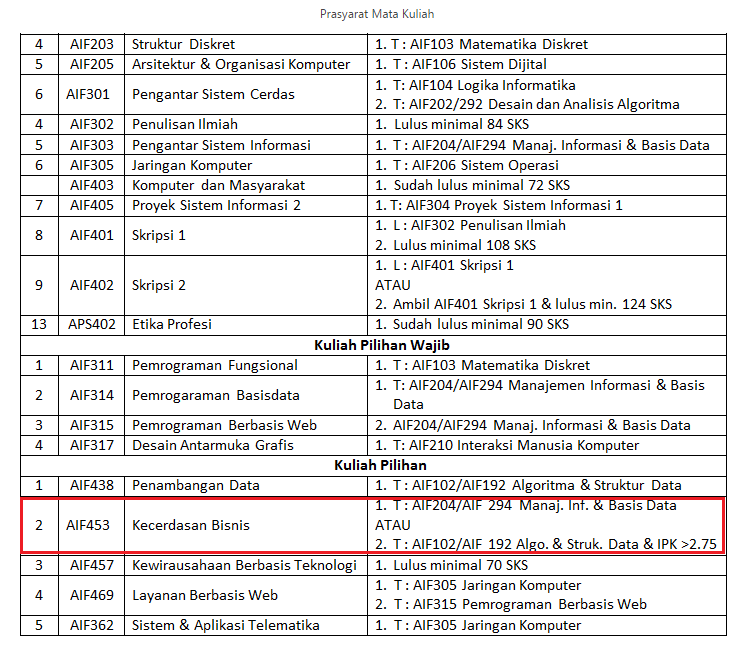
\includegraphics[scale=0.5]{Gambar/contoh-tinyurl}
	\caption{Prasyarat Mata Kuliah\cite{prasyaratIT}}
	\label{fig:1_prasyarat_tinyurl}
\end{figure}

\begin{figure}[H]
	\centering
	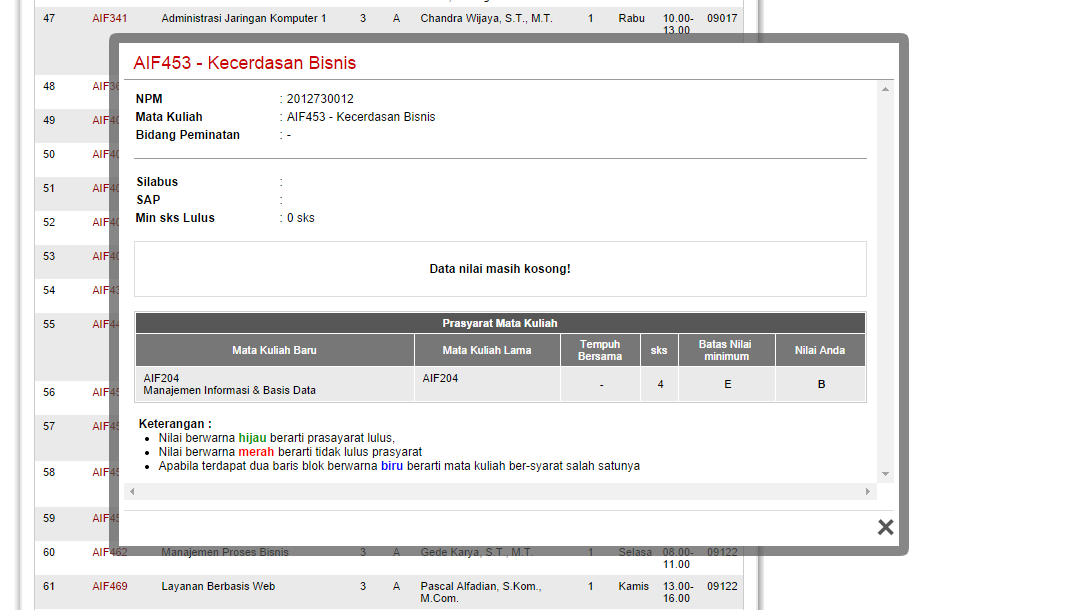
\includegraphics[scale=0.5]{Gambar/contoh-portal}
	\caption{Prasyarat Mata Kuliah Portal Akademik Mahasiswa\cite{studentportalunpar}}
	\label{fig:1_prasyarat_student_portal}
\end{figure}

Untuk mendukung kebutuhan akademik mahasiswa Program Studi Teknik Informatika, fitur-fitur yang diperlukan akan dianalisis kemudian diimplementasikan ke dalam sebuah aplikasi yang akan dinamakan Informatika Student Portal. Informatika Student Portal merupakan aplikasi berbasis web yang dibuat menggunakan Play Framework. Selain itu, data-data yang akan diolah diambil langsung dari Portal Akademik Mahasiswa dengan ekstraksi data situs web menggunakan \textit{library} jsoup. Untuk melakukan pengambilan data, jsoup harus mengetahui komunikasi dari Portal Akademik Mahasiswa. Analisis komunikasi Portal Akademik Mahasiswa akan dilakukan dengan menggunakan Chrome DevTools. 

\section{Rumusan Masalah}
\label{sec:rumusan_masalah}

Rumusan dari masalah yang akan dibahas pada skripsi ini adalah sebagai
berikut:
\begin{enumerate}
	\item Fitur-fitur apa saja yang dibuat untuk Informatika Student Portal?
	\item Bagaimana mengimplementasikan ekstraksi data situs web menggunakan \textit{library} jsoup?
	\item Bagaimana membangun aplikasi Informatika Student Portal?
\end{enumerate}

\section{Tujuan}
\label{sec:tujuan}

Tujuan-tujuan yang hendak dicapai pada skripsi ini adalah sebagai berikut:
\begin{enumerate}
	\item	Mendefinisikan fitur-fitur yang akan dibuat dalam Informatika Student Portal.
	\item	Mengimplementasikan ekstraksi data situs web menggunakan \textit{library} jsoup.
	\item Membangun aplikasi Informatika Student Portal.
\end{enumerate}

\section{Batasan Masalah}
\label{sec:batasan_masalah}

Beberapa batasan yang dibuat terkait dengan pengerjaan skripsi ini adalah sebagai berikut:
\begin{enumerate}
	\item Aplikasi akan diuji pada server FTIS sehingga tidak bisa diakses dari luar jaringan FTIS.
	\item Prasyarat mata kuliah yang tersedia hanya mata kuliah yang didukung SIA Models.
	\item Aplikasi tidak dapat menangani mahasiswa yang pernah melakukan transfer studi.
\end{enumerate}

\section{Metodologi Penelitian}
\label{sec:metode_penelitian}

Metodologi yang dilakukan pada skripsi ini adalah sebagai berikut:

\begin{enumerate}
	\item Melakukan studi mengenai \textit{library} jsoup untuk mengambil data dari Portal Akademik Mahasiswa, CSS Selector yang akan digunakan jsoup untuk menyeleksi data yang akan diambil, Chrome DevTools untuk menganalisis komunikasi Portal Akademik Mahasiswa, dan Play Framework untuk membangun Informatika Student Portal.
	\item Melakukan wawancara.
	\item Menganalisis Portal Akademik Mahasiswa.
	\item Merancang Informatika Student Portal.
	\item Mengimplementasikan ekstraksi data situs web menggunakan \textit{library} jsoup.
	\item Melakukan eksperimen dan pengujian.
	\item Membuat dokumentasi.
\end{enumerate}

\section{Sistematika Penulisan}
\label{sec:sistematika_penulisan}

Sistematika penulisan setiap bab pada skripsi ini adalah sebagai berikut:

\begin{enumerate}
  \item Bab Pendahuluan \\
  Bab 1 berisi latar belakang, rumusan masalah, tujuan, metode penelitian,
  dan sistematika penulisan yang digunakan untuk menyusun skripsi ini.
  \item Bab Dasar Teori \\
  Bab 2 berisikan teori-teori yang digunakan dalam pembuatan skripsi ini. Teori
  yang digunakan yaitu \textit{library} jsoup, Chrome DevTools, Play Framework, SIA Models, dan CSS \textit{selector}.
  \item Bab Analisis \\
  Bab 3 berisikan analisis yang dilakukan pada skripsi ini, meliputi analisis Portal Akademik Mahasiswa, analisis kebutuhan Informatika Student Portal, analisis komunikasi Portal Akademik Mahasiswa untuk fitur Informatika Student Portal, analisis \textit{use case} meliputi diagram \textsl{use case} dan skenario, serta analisis kelas. 
	\item Bab Perancangan \\
  Bab 4 berisikan perancangan aplikasi, meliputi diagram kelas rinci beserta deskripsi kelas dan fungsinya dan perancangan antarmuka aplikasi. 
	\item Bab Implementasi dan Pengujian \\
  Bab 5 berisikan implementasi dan pengujian aplikasi, meliputi lingkungan implementasi, hasil implementasi, pengujian fungsional, dan pengujian eksperimental.
	\item Bab Kesimpulan dan Saran \\
  Bab 6 berisikan kesimpulan dari hasil pembangunan aplikasi beserta saran untuk pengembangan berikutnya.
\end{enumerate}
